\chapter{Ansatz}

Im Storymodus des ctGameStudios lernen Schüler grundlegende Konzepte der Programmierung wie
Schleifen, Verzweigungen, Ereignisse, Prozeduren und Funktionen kennen. Der Storymodus ist in sich
geschlossen, da er einen festen Anfang und Ende hat, und im vornherein festgelegte, spezifische
Herausforderungen stellt.

Wir wollen das ctGameStudio erweitern, um Spielern die Möglichkeit und die Motivation dazu zu geben,
die im Storymodus gelernten Fähigkeiten anzuwenden und zu trainieren. Im Gegensatz zum Storymodus
soll dieser Spielmodus offen sein, so dass der Spieler seine Herausforderungen und Lösungsansätze
selbst bestimmen kann. Damit wiederholtes Spielen motiviert wird und die eigene Kreativiät gefördert
wird, sollen Herausforderungen durch sich selbst oder andere generiert werden können. 

Ein offener Spielmodus stellt die Fähigkeit in den Vordergrund, Problemstellungen zu analysieren,
und adäquate Problemlösestrategien zu entwickeln. Dadurch werden speziell die CT-Fähigkeiten der
Abstraktion und der Evaluation gefördert.

Inspiriert vom RoboCode und angelehnt an das letzte Level des Storymodus soll dieser Spielmodus aus
einem Roboterkampf bestehen. Es gilt, eine Strategie zu entwickeln, um die Strategie des Gegners zu
überwinden.

\section{Lernszenario}

Das Spiel soll solche Schüler unterstützen, die die Grundlagen der Programmierung kennen lernen und
ausbauen sollen. Der Kernlehrplan Informatik für Gymnasien und Gesamtschule in der Sekundarstufe
II\footnote{Kernlehrplan Informatik für Gymnasien und Gesamtschule in der Sekundarstufe II:
\cite{SchulministeriumNRW2014}} definiert als Inhaltsfeld die Entwicklung von Algorithmen, welche
als "genaue Beschreibung zur Lösung eines Problems" (S. 17) definiert werden. Dies entspricht der
Entwicklung von Problemlösestrategien in der Roboter-Mikrowelt des ctGameStudio, und zeigt, dass das
dieses Spiel die Anwendung in der Sekundarstufe II unterstützen sollte.

Folgendes Lernszenario soll darstellen, wie das Spiel die Ziele des Lehrplans unterstützt und in den
Unterricht eingebunden werden kann.

Um die Grundlagen des Spiels sowie die zur Entwicklung von Problemlösestrategien nötigen
Programmierkonzepte kennen zu lernen, spielen Schüler zunächst den Storymodus des ctGameStudio.
Durch Bearbeiten der Level des Storymodus werden die im Kernlehrplan definierten inhaltlichen
Schwerpunkte der Analyse, Entwurf und Implementierung einfacher Algorithmen (S. 23) unterstützt, und
anhand dessen die Kompetenzen des Argumentierens, der Modellierung, der Implementation, des
Darstellen und Interpretieren und Kommunizieren und Kooperieren gefördert.

Mit dem offenen Spielmodus werden die erlenten Kompetenzen vertieft. In Kämpfen zwischen dem eigenen
gegen einen Gegnerroboter entwickeln die Schüler eigene Kampfstrategien. Dabei können sie die
Gegnerstrategie aus eigenen oder vorgefertigten Strategien festlegen, um eine generell anwendbare,
gegen viele Herausforderungen effektive Strategie zu entwickeln. Nachdem die Schüler eine oder
mehrere Strategien entwickelt haben, kann der Lehrer ein Turnier veranstalten, in dem die Strategien
gegeneinander ausgespielt werden und eine Rangliste entsteht. Das Turnier wird an einem gemeinesamen
Bildschirm oder Projektion verfolgt, und liefert eine Diskussionsgrundlage um Strategien gemeinsam
zu evaluieren. In weiteren Durchgängen können Schüler ihre Strategie verbessern, und weitere
Turniere veranstaltet werden.


\section{Offener Spielmodus: RoboStrategist}

Kern des offenen Spielmodus ist der Kampf zwischen zwei Robotern, die vorprogrammierte Strategien
ausführen. Die Strategien sind Algorithmen zur Koordination der Fähigkeiten des Roboters, um den
Gegner Schaden zuzufügen, und eigenen Schaden zu vermeiden. Eine erfolgreiche Strategie besteht aus
effektiver Positionierung des Roboters auf dem Spielfeld, dem Ausweichen von Schüssen nachdem man
getroffen wurde, dem Ausfinding machen und Verfolgen des Gegners, und das Zielen und Schießen auf
den Gegner.


\subsection{Training}

Der Training fördert eigenständiges, selbst-geleitetes Lösen von Problemen, und bietet damit
eine Plattform, seine Programmierfähigkeiten zu vertiefen. Zum Einen werden komplexe
Herausforderungen in Form von unterschiedlichen Gegnerstrategien gestellt. Der Spieler
wendet Abstraktionen wie Schleifen, Verzweigungen, Variablen, Prozeduren und Funktionen an, um einen
Algorithmus zu entwickeln. Der Algorithmus ist das Code-Artefakt, das gegen das Problem in Form der 
Gegnerstrategie evaluiert wird.

Zum Anderen kann der Spieler eigenständig wählen, wie er bei der Entwicklung der
Problemlösestrategie vorgeht, in dem er selbst wählt, gegen welche Strategien er seine Strategie
testet. Im Rahmen dieser Arbeit sollen dafür dafür drei vorgefertigte Gegnerstrategien verfügbar
sein. Die Strategien unterscheiden sich in ihren Ansätzen, ihrer Komplexität, und der Schwierigkeit,
sie zu besiegen.

Die erste Strategie, \enquote{Verwirrt}, (Abb. \ref{strategie-verwirrt}) ist dazu gestaltet, einen
einfachen Einstieg in die Strategieentwicklung zu geben. Der Roboter bewegt sich in zufälligen
Zeitabständigen auf zufällig gewählte Positionen, und gibt zwischendurch Schüsse in zufällige
Richtungen ab. Um den Roboter zu besiegen, muss der Spieler eine Strategie entwickeln, die den
Gegner immer wieder auffindet, und Schüsse in seine Richtung feuert. Dadurch, dass kein
Zielen auf den Roboter des Spielers besteht, muss die Lösungsstrategie nicht besonders effizient
sein. Auch um die eigene Positionierung muss sich der Spieler keine Gedanken machen.

\begin{figure}
  \centering
  \label{strategie-verwirrt}
  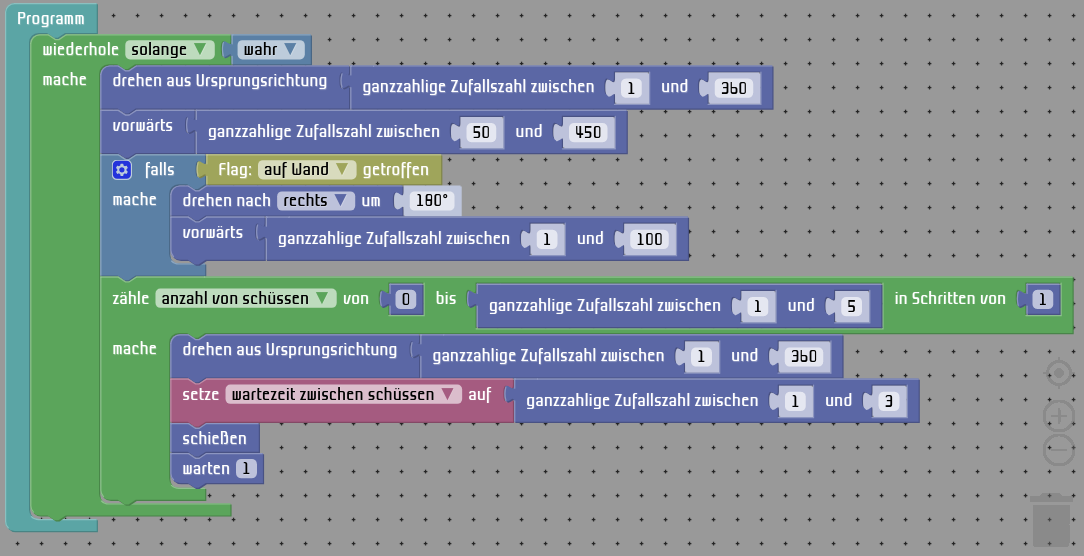
\includegraphics[scale=1, keepaspectratio]{figures/strategy-verwirrt.png}
  \caption{Blockly-Sicht der \enquote{Verwirrt}-Strategie}
\end{figure}

Die zweite Strategie, \enquote{Wandkrabbler} (Abb. \ref{strategie-wandkrabller}), agiert in einem
vorsehbaren Muster. Der Roboter bewegt sich an am Spielfeldrand entlang und scannt in kleinen
Abständen voneinander entgegengesetzt der Wand nach dem Gegner. Wurde dieser entdeckt, schießt er
solange, bis der Gegner seine Position ändert. Diese Strategie erfordert vom Spieler eine Strategie
zu entwickeln, in der unterschiedliche Postionen eingenommen werden, um die Entdeckung durch den
Gegner zu verzögern und im Fall eines Treffers weiteren Schüssen auszweichen. Die erhöhte Gefahr
durch den Wandkrabbler erfordert auch einen effizienten Scanvorgang, so dass man den Gegner öfter
und schneller auffindet und Schaden zufügt, als er es tut.

\begin{figure}
  \centering
  \label{strategie-wandkrabbler}
  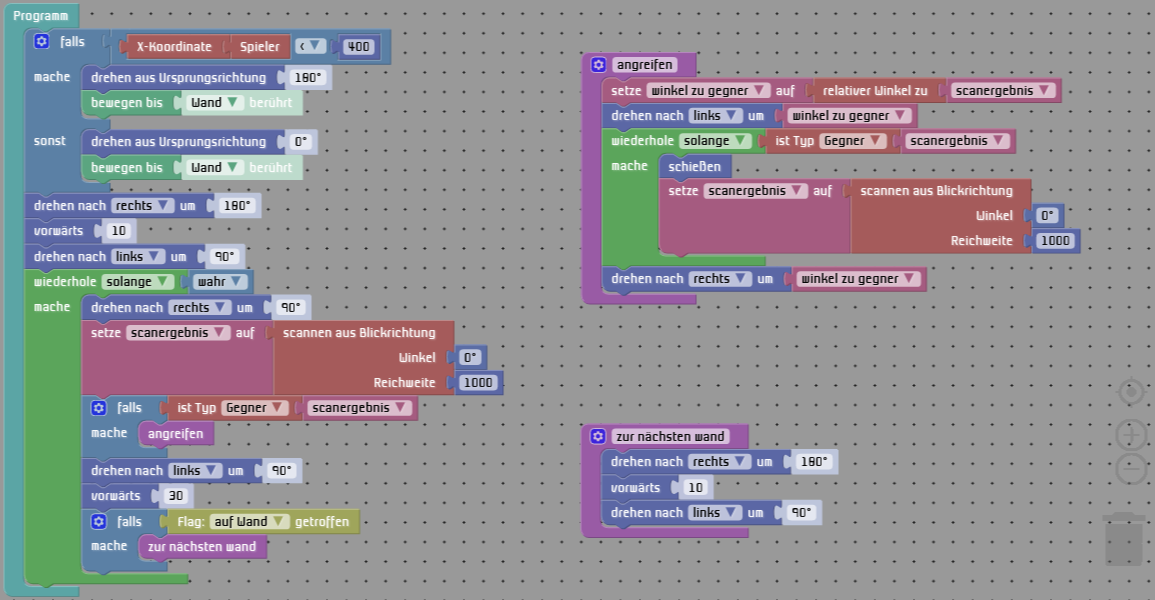
\includegraphics[scale=1, keepaspectratio]{figures/strategy-wandkrabbler.png}
  \caption{Blockly-Sicht der \enquote{Wandkrabbler}-Strategie}
\end{figure}

Die dritte Strategie, \enquote{Eckenschütze} (Abb. \ref{strategie-sniper}), ist die
gefährlichste aller Strategien. Zunächst hat sie den effizientesten Scanmechanismus. Dazu bewegt der
Roboter sich zwischen den Ecken des Spielfelds, und scannt von den Ecken aus in kleinen Schritten
das gesamte Spielfeld ab. So ist die Chance groß, innerhalb eines kurzen Zeitraums den Gegner
aufzufinden. Wurde der Gegner entdeckt, werden so lange Schüsse abgegeben, bis der Gegner seine
Position ändert. Die Strategie implementiert zudem einen Ausweichmechanismus, so dass der Roboter in die
nächste Ecke wechselt, wenn er getroffen wurde. Um diese Strategie zu besiegen erfordert ständige
Bewegung auf dem Spielfeld, um den Scanvorgängen zu entgehen. Wahrscheinlich sollte sie ein eigenen
Ausweichmechanimus implementieren, und einen effiziente Scanvorgang beinhalten.

\begin{figure}
  \centering
  \label{strategie-sniper}
  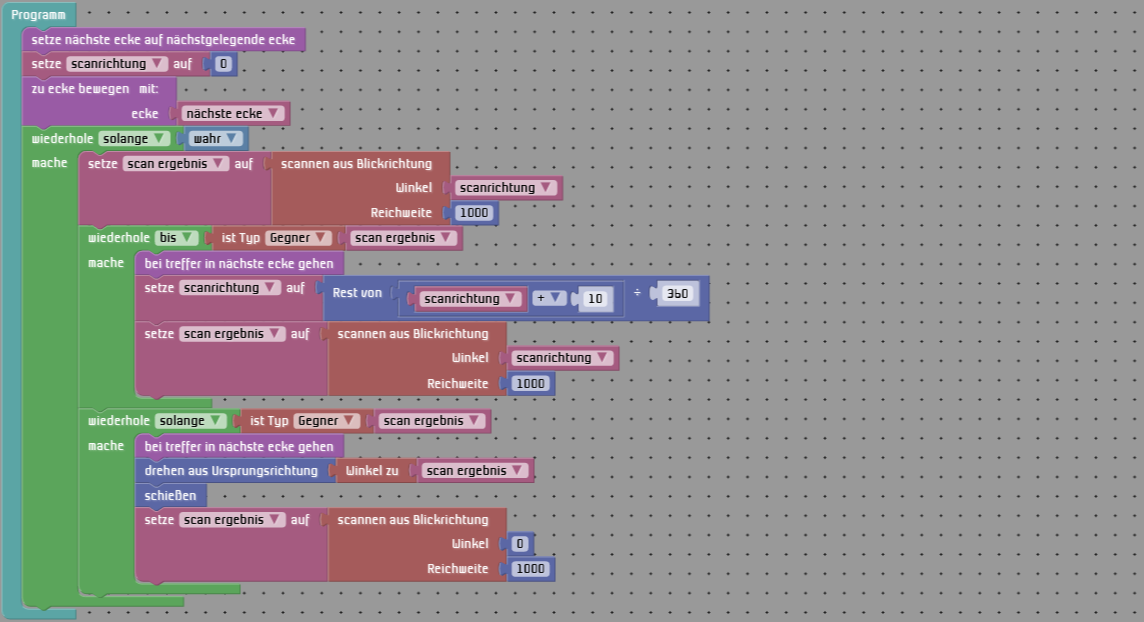
\includegraphics[scale=1, keepaspectratio]{figures/strategy-sniper-1.png}
  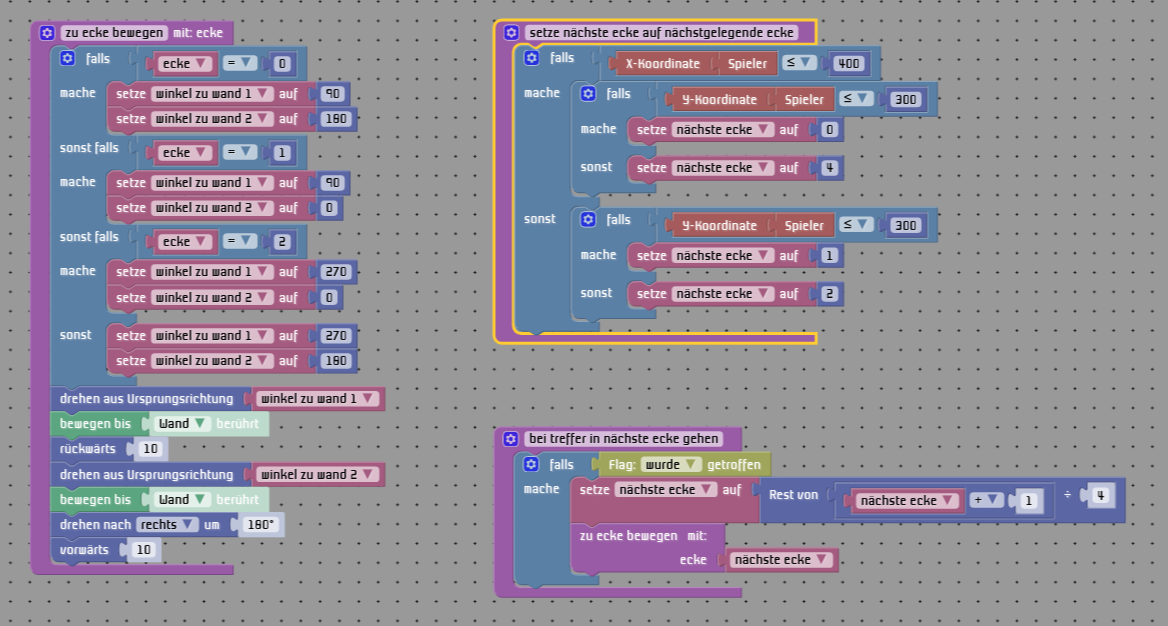
\includegraphics[scale=1, keepaspectratio]{figures/strategy-sniper-2.png}
  \caption{Blockly-Sicht der \enquote{Eckenschütze}-Strategie}
\end{figure}

Wie bereits vorgestellt sollte eine Mikrowelt nach Papert ein iteratives, selbst gesteuertes Vorgehen
erlauben, um die inherente Kreativität und Explorationswillen des Menschen zu nutzen. In diesem
Sinne wollen wir dem Spieler die Möglichkeit geben, als Gegnerstrategien neben den vorgefertigten
auch selbst erstellte Strategien zu wählen. Um seine Strategie zu verbessern, könnte der Spieler
durch eine Analyse Schwachpunkte seiner Strategie feststellen, und versuchen diese mit einer neuen
Strategie konkret auszunutzen.

Das eigenständige, selbst-geleitete Lösen von Problemen soll einen kreativen Lösungsprozess des
Spielers fordern, ein exploratives Vorgehen motivieren, und damit verglichem mit dem geleiteten
Prozess des Storymodus einen höheren Lerneffekt erzielen.

Folgendes Schema stellt eine neue Strategieentwicklung dar.
% und zeigt, dass die Entwicklung einer Strategie im Training den drei Stufen des Compuational Thinking Prozesses \ref{repenning_principles_2017}

\begin{enumerate}
\item Die initial geladenene Gegnerstrategie wird ausgeführt.
\item Man analysiert die Gegnerstrategie und bildet erste Lösungsansätze (Problem Formulation).
\item Man formuliert und implementiert erste Lösungsansätze (Solution Expression). Man kann auf das Wissen aus den letzten
Leveln des Storymodus zurückgreifen, um einen ersten Anhaltspunkt dafür zu haben.
\item Man führt den Kampf aus und analysiert seinen Verlauf (Solution Execution \& Evaluation). Die Evaluationskriterien sind, ob der Roboter
das macht, was man mit dem Programm erzielen wollte, und ob der Problemansatz zum Erfolg führt.
\item Aufgrund der Analyse verbessert der Spieler seine Strategie.
\item Schritt 4 und 5 werden wiederholt, bis der Gegner wiederholt geschlagen werden kann.
\item Der Spieler wählt eine neue Gegnerstrategie.
\item Schritt 4 bis 7 werden wiederholt, bis der Spieler alle Gegnerstrategien hat. Der Spieler kann außerdem
versuchen, seine eigene Strategie zu besiegen, in dem er sie als Gegnerstrategie festlegt.
\end{enumerate}

Um verschiedene Strategieansätze ausprobieren zu können, und in mehreren Sitzungen an den Strategien
arbeiten zu können, kann der Spieler seine Strategien speichern, kopieren, neue anlegen, und
zwischen diesen wechseln.


\subsection{Turniere}

Turniere sind spannend und erhöhen Spielspaß und damit die Motivation, das Spiel zu spielen. Der
kompetitive Aspekt wird Spieler dazu motivieren, gute Strategien zu entwickeln. Die
Turnierdurchführung selber bietet einen Vergleich zwischen Strategien und ist so
Diskussionsgrundlage für verschiedene Strategieansätze und Verbesserungen.

Da es verschiedene Möglichkeiten gibt, ein Turnier durchzuführen, und diese ihre eigenen Vor- und
Nachteile haben, wollen wir dem Turnierveranstalter die Wahl eines Turniersystems geben. In dieser
ersten Version des Open Stage-Modus wollen wir die zwei gebräuchlisten Turniersysteme zur Wahl
stellen.

Das Jeder-gegen-Jeden-System ist die ausführlichste Weise, ein Turnier durchzuführen. Ein Beispiel
für diese Turnierart ist die deutsche Fußballbundesliga. Um in diesem System eine Rangfolge zwischen
Teilnehmern zu erzielen, tritt jeder Teilnehmer gegen jeden anderen Teilnehmer an und zählt die
Siege, die erreicht wurden. Vorteil ist, dass diese Rangfolge erschöpfend ist. Nachteil dieses
Modus ist die quadratisch steigende Anzahl von Kämpfen ($n x n$ Kämpfe bei $n$ Teilnehmern),
die durchgeführt werden müssen. Für die Evaluation von Strategien im Open Stage-Modus bietet sich das
Jeder-gegen-Jeden-System an, wenn eine geringe Anzahl von Teilnehmern besteht.

Das KO-System ist eine effizientere Weise, ein Turnier durchzuführen. Ein Beispiel für diese
Turnierart ist die KO-Phase eines Fußball-Weltmeisterschaft. Das Turnier verläuft in Runden, wobei
in der ersten Runde zufällig ausgewählte Pärchen gegeneinander antreten. Während der Verlierer eines
Kampfes vom Turnier ausscheidet, geht der Sieger in die nächste Runde. Vorteil dieses Turnieres ist,
dass gegenüber dem Jeder-gegen-Jeden-System weitaus weniger Kämpfe ausgeführt werden ($n - 1$ Kämpfe
bei $n$ Teilnehmern). Außerdem hat dieser Modus einen interessanteren Spannungsbogen, da bei jedem
Kampf ein Spieler ausscheidet, und nach jeder Runde die Anzahl der Spieler durch zwei geteilt wird,
bis es am Ende ein spannendes Finale gibt. Nachteil dieses Systems ist, dass die aus dem Turnier
resultierende Rangfolge nicht zwangsläufig repräsentativ für die tatsächliche Rangfolge der
Strategien ist. So mag es beispielsweise sein, dass die Gewinnerstrategie bei einem Turnier mit acht
Teilnehmern eigentlich gegen vier der sieben Gegner verlieren würde, durch die zufällige initale
Paarung jedoch auf die drei übrigen Strategien getroffen ist. Während er in dieser Paarung das
Turnier gewinnen könnte, wäre er im Jeder-gegen-Jeden-Modus nicht zwangsläufig an oberster Stelle
der Rangliste. Ein weiterer Nachteil ist, dass ein faires Turnier im KO-Modus mit mehr als zwei
Teilnehmern eine Teilnehmeranzahl haben muss, die durch vier teilbar ist. Da dies nicht immer
möglich ist, wollen wir dem Veranstalter die Möglichkeit geben, fehlende Teilnahmen durch selbst
festgelegte Strategien aufzufüllen. Für die Evaluation von Strategien im Open Stage-Modus bietet
sich bei einer hohen erwarteten Anzahl von Teilnehmern an, und der Unterhaltungswert des Turniers
eine große Rolle spielt. 

Wenn Strategien ineffektiv sind, kann es sein, das in einem Kampf innerhalb eines vertretbaren
Zeitraums kein Sieger festegestellt werden kann. Deshalb soll bei Erstellung des Turniers eine
maximale Rundendauer festgelegt werden können. Im Jeder-gegen-Jeden-Modus geht der Kampf nach Ablauf
der Zeit unentschieden aus. Im KO-Modus muss ein Sieger festgestellt werden. Dauzu gewinnt in
diesem Modus nach Ablauf dieser Zeit der Spieler, dessen Roboter weniger Schaden genommen hat. Sind
hier beide Spieler gleich, kann der Turnierleiter selbst einen Sieger festlegen.

Da bereits zu vor Ablauf der Zeit absehbar sein kann, dass es zu keinem Sieger kommen wird, soll es
außerdem es die Möglichkeit geben, eine Runde abzubrechen. Der Turnierleiter kann den Kampf
wiederholen, oder das Ergebnis selbst bestimmen.

Das Resultat mehrerer Kämpfe mit den selben Strategien kann aufgrund der zufälligen Startposition
der Roboter unterschiedlich sein. Um die tatsächliche bessere Strategie zu ermitteln, könnte es
nötig sein, einen Kampf aus mehreren Runden bestehen zu lassen. Ein Spieler würde dann den Kampf
gewinnen, der zuerst zwei oder drei Runden gewonnen hat. Auch hierfür soll es bei Erstellung des
Turnieres eine Option geben.

Die Turnierfunktion ist so gestaltet, dass die Teilnehmer nicht bei Erstellung des Turniers bekannt
sein müssen. Dazu wird bei Erstellung einen Zugangscode generiert. Spieler, die diesen Code kennen,
können sich mit einer ihrer im Training erstellten Strategien am Turnier anmelden.

In einer Turnierliste kann der Turnierersteller die Namen und Strategienamen der Teilnehmer
einsehen, und das Turnier starten. Um die Durchführung des Turniers zu verfolgen muss der Bildschirm
des Turniererstellers betrachtet werden.

Eine Turnierübersicht zeigt den Verlauf und Ranglisten des Turniers. Die Ansichten unterscheiden
sich dabei je nach Turniersystem. Im Jeder-gegen-Jeden-Modus werden vergangene Kämpfe, noch
anstehende Kämpfe, und eine Tabelle mit der Anzahl von Siegen pro Spieler angezeigt. Im KO-Modus
wird der Turnierbaum angezeigt. Der Turnierersteller kann den jeweils nächsten Kampf über einen
Button starten. Das Spielfeld wird geladen und der Kampf ausgeführt. Nach Ende des Kampfes wird die
aktualisierte Turnierübersicht dargestellt.


\section{Anforderungsanalyse}

Zur Implementation des Open Stage-Modus muss das Benutzerinterface um Dialoge und Menüs zur Auswahl
des Spielmodus und der Erstellung, Teilnahme an und Durchführung von Turnieren erweitert werden.

Das Spiel soll um ein Strategiemanagement erweitert werden, um Strategien über mehrere Sitzungen
hinweg bearbeiten zu können, und gleichzeitig Zugriff auf mehrere Strategien zu haben, die getrennt
voneinander evaluiert und bearbeitet werden können.

Die Spielfläche muss durch einen zweiten, durch eine nutzerdefinierte Strategie gesteuerten Roboter
mit eigener Lebensanzeige, erweitert werden. Die Interaktion zwischen den Robotern muss so gestaltet
werden, dass unterschiedliche Ansätze zwischen Strategien (z.B. ein Fokus auf viel Bewegung,
effizientes Scannen oder Ausweichen) erfolgsversprechend sein können. Das Geschwindigkeit des
Gameplays sollte so angepasst werden, dass die Interaktion der Roboter und ihre Bewegungen gut
nachvollziehbar sind. Für die Turnierdurchführung muss das Spielfeld außerdem um eine
Benutzeroberfläche zum Abbruch von Kämpfen und eine Anzeige der verbleibenden Zeit und Rundenzahl
erweitert werden. 

Als zusätzliches Ziel soll die Konzeption und Umsetzung eines immersiven, thematisch passenden
Designs gesetzt werden, damit der Fantasy-Aspekt des Spiels und der allgemeine Spielspaß gestärkt
wird.
